\section{Re-construction of Descriptive Patterns}
\begin{figure}[!h]
\centering
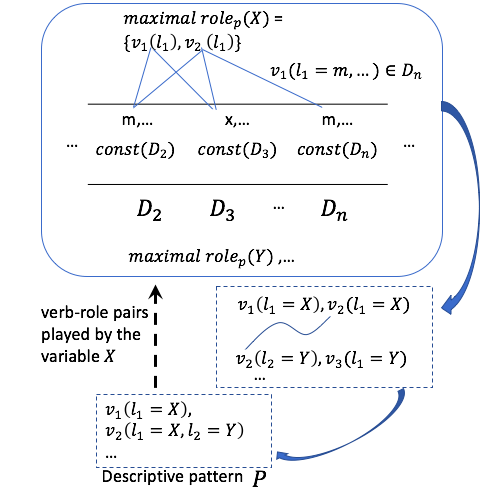
\includegraphics[width=250pt]{./pictures/0306.png}
\caption{primitive patterns and closures}
\end{figure}
If a pattern $P  = \{...,p(...,l = X,...),...\}$ can be a descriptive pattern, it should be with a maximal role set of variables $X,...(role_p (X),...)$ , and it should meet the condition of minisup. Using a Formal Concept Analysis Algorithm we can get the maximal closure $role_P (X)$ of the target descriptive pattern. The $role_P (X)$ meet the condition of minsup the descriptive pattern re-construct by it will also meet the condition of minsup. We can explain our idea in a figure.\\
We  have primitive pattern for closures,
\begin{displaymath}
pp(X) = v_1(l_1 = X), v_2(l_1 = X),...
\end{displaymath}
Although extracting all descriptive patterns will be a very difficult work depending on the document set we choose, by enlargement of role set and get maximal closures of $role_P (X)$ , the argument in $pp(X)$ is extended. That means more specific patterns can be extracted. Every possible specific pattern can be extracted from closures.\\
\begin{figure}[!h]
\centering
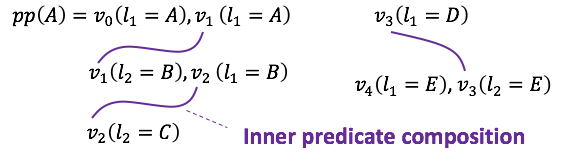
\includegraphics[width=300pt]{./pictures/0306-1.png}
\caption{Inner predicate composition}
\end{figure}
We have talked about the degree of difficulty to extract all descriptive patterns from maximal closure, but we can generate some representative descriptive pattern by some method. We have introduced KeyGraph Algorithm in the chapter before. And understand the association value between different nouns. Connecting same verbs in the primitive pattern set means to find a strong connection between the nouns, we always connect the highest association value pair one by one, until we cannot find other connections, we can understand this process in a figure.\\
Here is the detail process for this part, re-construct descriptive patterns $P$ with maximal closure set $C$.\\
We have a maximal closure set, We will have the primitive pattern for each closure.\\
\begin{displaymath}
pp(X) = v_1(l_1 = X), v_2 (l_1 = X)...
\end{displaymath}
\begin{displaymath}
pp(Y) = v_2(l_2 =Y),...
\end{displaymath}
Our purpose is to connect the verb-cases in primitive patterns to build the descriptive pattern. For each variable:
\begin{displaymath}
X, Y,... :X = {x_1, x_2,....}
\end{displaymath}
First we should find all the workable connections:
\begin{displaymath}
v1:\{\},v2:\{X,Y\},...
\end{displaymath}
We define the distance of the variables as the association value defined by KeyGraph Algorithm,
\begin{displaymath}
distance(X, Y) = \sum_{x_i \in X, y_i \in Y} association(x_i, y_i)
\end{displaymath}
Rank the value of distance, connect the strongest one. Then kick out the connected ones, repeat the process again. Finishing the whole processing, we will get one descriptive pattern if we always choose the strongest connection from our maximal closure set.\\
As the inner predicate composition is just a recover of the co-occurrence of nouns, we can use a breadth first algorithm to extract all possible descriptive patterns. The breadth first algorithm may take a large space and runtime, we propose beam search algorithm to help us pikc some main descriptive pattern from some sense.
As the association value recover the co-occurrence of nouns we have introduced, we also explained the Beam Search Algorithm in the former section. we can combine them together to get more than one Descriptive Patterns form a maximal closure set.\\
\begin{figure}[!h]
\centering
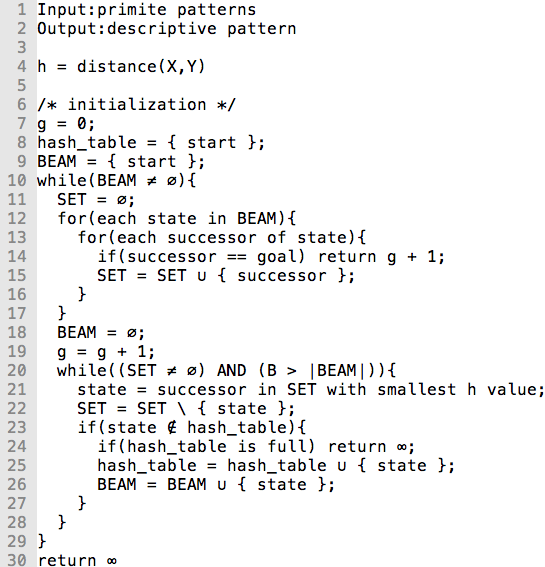
\includegraphics[width=250pt]{./pictures/0306-2.png}
\caption{Beam Search for re-construct descriptive patterns}
\end{figure}
